\chapter{LOWESS}

% TODO: add "weighted average" material somewhere.
% TODO: and example of "average of averages" not being the true average (if
% group sizes are different.)

\index{noise}

A common exploratory technique for bivariate, numerical data involves finding a
smooth curve to approximate a noisy data set. The structure of the data -- and
whether there even is a relationship between the two variables at all -- may be
more easily visible from such a curve than from a raw splattering of points.

\section{Best-fit line: ``parametric''}

\index{best-fit line}
\index{least-squares line}
\index{line, best-fit / least-squares}
\index{polyfit@\texttt{polyfit()} (NumPy)}
\index{sort@\texttt{.sort()} (NumPy)}

In your stats class, you probably learned how to compute the best-fit line
to a set of bivariate numerical data points, where ``best fit'' was taken in a
``least squares'' sense (\textit{i.e.}, the line that minimizes the sum of the
squared deviations of the line from the actual data points). It will not
surprise you that it's easy to do this in Python as well, as
shown in Figure~\ref{fig:bestFitCode} (p.~\pageref{fig:bestFitCode}).


\index{polyfit@\texttt{polyfit()} (NumPy)}
\index{polynomial}

NumPy's ``\texttt{polyfit()}'' function stands for ``polynomial fit.'' You'll
recall from high school algebra that a polynomial is a function that involves
only \textit{powers} of your $x$ variable: squares, cubes, and so forth (no
sines, cosines, logarithms, ``$e$-to-the's'' or anything else). Also permitted
are a plain-old $x$ term (since that's $x^1$, or ``$x$ to the first power'')
and a constant term (since that's $x^0$, or ``$x$ to the zeroth power''). And
any of these things can be multiplied by any coefficient you like. So, one
example polynomial would be:

\begin{align*}
y = 4.3 x^3 - 29.4 x^2 + 6 x - 13.8
\end{align*}
\vspace{-.25in}

\index{degree (of a polynomial)}
\index{coefficients (of a polynomial)}

The \textbf{degree} of a polynomial is the highest exponent it contains; this
example has degree 3.

\bigskip
\begin{figure}[hb]
\begin{Verbatim}[fontsize=\footnotesize,samepage=true,frame=single,framesep=3mm]
# Create x points and some crazy, noisy y function of them.
x = np.random.uniform(0,100,100)
x.sort()
y = 4*x - .2 * x**2 + np.random.normal(0,120,100)

# Get the slope and intercept of the best-fit line.
m, b = np.polyfit(x, y, 1)

# Heck, while we're at it let's find the best-fit quadratic too.
a1, a2, a3 = np.polyfit(x, y, 2)

# Plot the points and the approximations.
plt.scatter(x,y)
plt.plot(x, m*x + b,color="green")
plt.plot(x, a1*x**2 + a2*x + a3,color="purple")
\end{Verbatim}
\caption{Finding and plotting the best-fit (least-squares) line. (Note that we
have to \texttt{.sort()} the $x$ points since we draw line plots based on
them, and you get crazy zig-zags if you don't sort your $x$ values first.)}
\label{fig:bestFitCode}
\end{figure}
\bigskip
 

Now the \texttt{polyfit()} function asks: which polynomial can I pick (of a
given degree) that will get the closest to the data points -- \textit{i.e.},
minimize the squared distances between the polynomial's value and the points?
It takes three arguments: an array of $x$ values, an array of $y$ values, and
the degree. It returns the coefficients for the best-fit polynomial of that
degree. So in the Figure~\ref{fig:bestFitCode} code, this line:

\begin{Verbatim}[fontsize=\small,samepage=true,frame=single,framesep=3mm]
m, b = np.polyfit(x, y, 1)
\end{Verbatim}

says ``please give me the coefficients of the best-fit 1-degree polynomial to
these \texttt{x} and \texttt{y} points.'' Since a 1-degree polynomial is a
straight line, we got two coefficients back, which we named \texttt{m} and
\texttt{b}, as is traditionally done. Plotting the actual line was accomplished
with this code:

\begin{Verbatim}[fontsize=\small,samepage=true,frame=single,framesep=3mm]
plt.plot(x, m*x + b,color="green")
\end{Verbatim}

\index{y=mx+b@$y=mx+b$}

which says ``For each $x$ value in the data set, plot $x$ versus $mx+b$.'' And
that, of course, plots the line with slope \texttt{m} and $y$-intercept
\texttt{b}. Similar code plots the best-fit quadratic function (2-degree
polynomial), or any degree we like.

\index{parametric model}

No matter what degree we use, these approximations are called
\textbf{parametric} models because they're based on (global) parameters: a
slope and an intercept, say, or three coefficients in the case of the
quadratic. In each case, we assume the data fit an overall particular
``functional form'' (like a line, or a quadratic) and say, ``given that we feel
like these data are `really' a line, what parameters that describe a line would
give us the best line?''

Figure~\ref{fig:bestFitPlot} (p.~\pageref{fig:bestFitPlot}) shows the best-fit
line and best-fit quadratic (function with an $x^2$ term) for the points
generated by the code in Figure~\ref{fig:bestFitCode}.

\begin{figure}
\centering
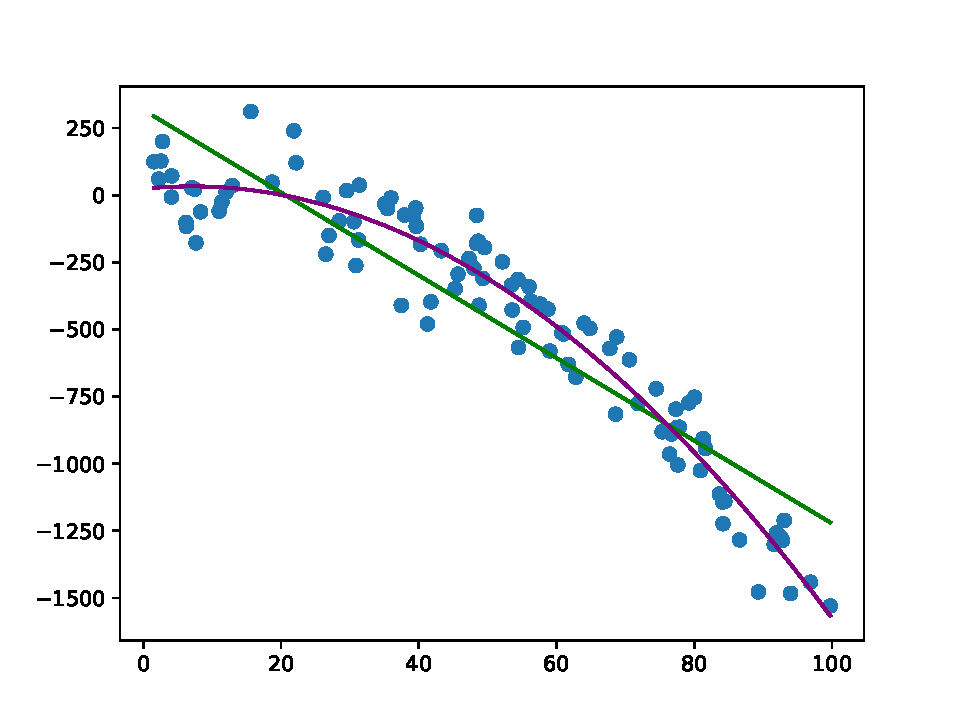
\includegraphics[width=0.8\textwidth,
  alt={Scatter plot of about 100 blue points sloping downward from near 0 at x = 0 to about -1500 at x = 100, curving more steeply toward the right, with two fitted curves: a green straight least-squares line, and a purple least-squares quadratic that bends to follow the points.}]{bestfit.pdf}
\caption{The best-fit line, and best-fit quadratic, to the set of points
generated by the code in Figure~\ref{fig:bestFitCode}.}
\label{fig:bestFitPlot}
\end{figure}
\section{LOWESS: ``non-parametric''}

A more sophisticated technique for this task is called ``\textbf{LOWESS}''
(sometimes ``\textbf{LOESS}''\footnote{Some authors make a very fine
distinction between the LOESS and the LOWESS techniques, which is too nitpicky
to even get into here. We'll treat the two terms as synonymous.}), which
(sorta) stands for ``Locally Weighted Estimated Scatterplot Smoothing.''
LOWESS tries to capture the overall trend of a messy set of data -- but what
distinguishes it from a best-fit line is that it operates \textit{locally}
rather than globally. When you crunch the numbers to find the best-fit
least-squares line to a data set, you're asking, ``what values of slope and
intercept for a \textit{single} line across the \textit{entire} data set will
give me the lowest \textit{overall} deviation from the points?'' (The same is
true for a best-fit quadratic, cubic, \textit{etc.}) In other words, you're
attempting to fit a single model over the entire range of data, and penalizing
inaccuracies equally everywhere.

By contrast, the LOWESS technique approximates the data \textit{locally}. This
means that it weights the data points in such a way that points close to the
location of interest contribute more strongly than do data points farther
away. It does this by fitting a linear (or polynomial) regression to each $x$
point of interest, but using a weighted contribution from only the nearby
points.

Here's how it works. We start with a bunch of $(x,y)$ points, and we want to
compute a ``locally smoothed'' $y$ for every one of the $x$'s. 

First, we have a parameter $\alpha$ that specifies \textit{what fraction of
the data} to take into account (at all) for each estimate. This can be any
value from 0 to 1. You might guess that the smaller it is, the more wiggly
it'll allow our smoothed estimate to be, since we'll be considering only a
small number of points. This is true, as we'll see.

Then, once we've fixed $\alpha$, we're going to find a bunch of best-fit,
least-squares lines, one at each $x$ value. This is just like in regular old
linear regression. The catch is that instead of minimizing the \textit{sum} of
squared differences, we're going to minimize the \textbf{weighted} sum. And
we'll place a greater weight on the errors for $x$ points close to the one
we're evaluating. This will have the effect of allowing the curve to bend
closely to our actual data points while ignoring stuff that's far away.

Written in equations, the ordinary best-fit line approach finds an $m$ and $b$
that minimize the overall sum of squared deviations (or ``residual sum of
squares''):

\begin{align*}
RSS = \sum_i (y_i - (mx_i + b))^2
\end{align*}

But with LOWESS, we calculate this separately for every $x$ point, and we
weight this with a \textbf{weight function} $w$:

\begin{align*}
RSS(x) = \sum_i w(x-x_i) \cdot (y_i - (mx_i + b))^2
\end{align*}

Note how the weight function is given the distance between the $x$ value of
interest and the locations of the actual data points. Since we want to weight
close-by points more heavily, the $w$ should be higher for values closer to
zero.\footnote{\index{kernel} If you're really on your game, you might observe
that the weight function is much like the \textit{kernel} for KDEs: in fact, it
really is basically a kernel. \index{Gaussian (kernel)} Thus we can use a
Gaussian for it, just like we did for KDEs, although it's more common with
LOWESS to use the so-called ``tri-cube'' kernel: $w(\Delta x) = (1 - |\Delta
x|^3)^3$ for $|x|<1$ (and 0 otherwise).}

This is \textbf{non-parametric} because when we're done, if somebody asked,
``hey, I like your LOWESS curve -- what parameters did you use for it?'' the
answer would be ``uh...there really aren't any parameters.'' The curve is a
messy combination of a bunch of different shifting approximations that we
calculated as we went through the whole data set. We didn't choose parameters
to plug into a particular model; in fact, we didn't really \textit{have} a
model.

Like KDEs, this technique wasn't computationally possible until the age of
computers. Hence it's one of the newer kids on the block. Here's how to do it
in Python with the \texttt{statsmodel} library:

\index{import@\texttt{import}}

\begin{Verbatim}[fontsize=\footnotesize,samepage=true,frame=single,framesep=3mm]
from statsmodels.nonparametric.smoothers_lowess import lowess

l = lowess(y,x,frac=1/3)
plt.plot(l[:,0],l[:,1],color="red")
\end{Verbatim}

\index{bias-variance trade-off}
\label{bvTradeoffLowess}

The ``\texttt{frac}'' parameter is our $\alpha$. The resulting curve for two
different values of $\alpha$ is shown in Figure~\ref{fig:lowess}. Notice how
$\alpha = \frac{1}{3}$ gives a much smoother line than $\alpha =
\frac{1}{10}$, since it is using more points to do the smoothing. In fact, the
former is quite close to the best-fit quadratic in this case. This is a
manifestation of the classic ``bias-variance trade-off'' we'll look closely at
in Chapter~\ref{ch:kNN2}.

\begin{figure}[ht]
\centering
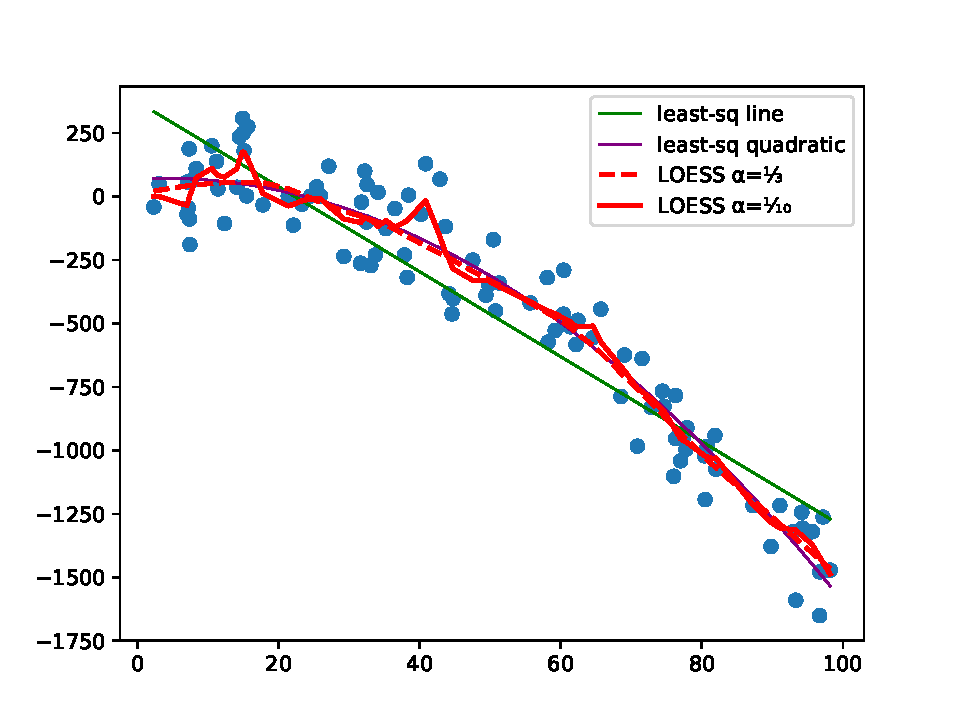
\includegraphics[width=1\textwidth,
  alt={The same noisy downward-curving scatter with four fitted curves per the legend: green least-squares line, purple least-squares quadratic, dashed red LOESS with alpha one third, and solid red LOESS with alpha one tenth. The quadratic and both LOESS curves track the points closely, the alpha one tenth curve with small wiggles.}]{lowess.pdf}
\caption{Various attempts to plot the ``true, underlying pattern'' of our
noisy data set.}
\label{fig:lowess}
\end{figure}

\smallskip

LOWESS might not appear to have much of an advantage over just a plain old
line. But Figure~\ref{fig:lowessBetter} (p.~\pageref{fig:lowessBetter}) shows a
data set where neither the line nor the quadratic are even in the ballpark, yet
where LOWESS does quite well. Intuitively, if the data \textit{aren't}
ultimately generated by something linear (or close to it), a linear model will
be hard-pressed to capture the curve.

\begin{figure}[ht]
\centering
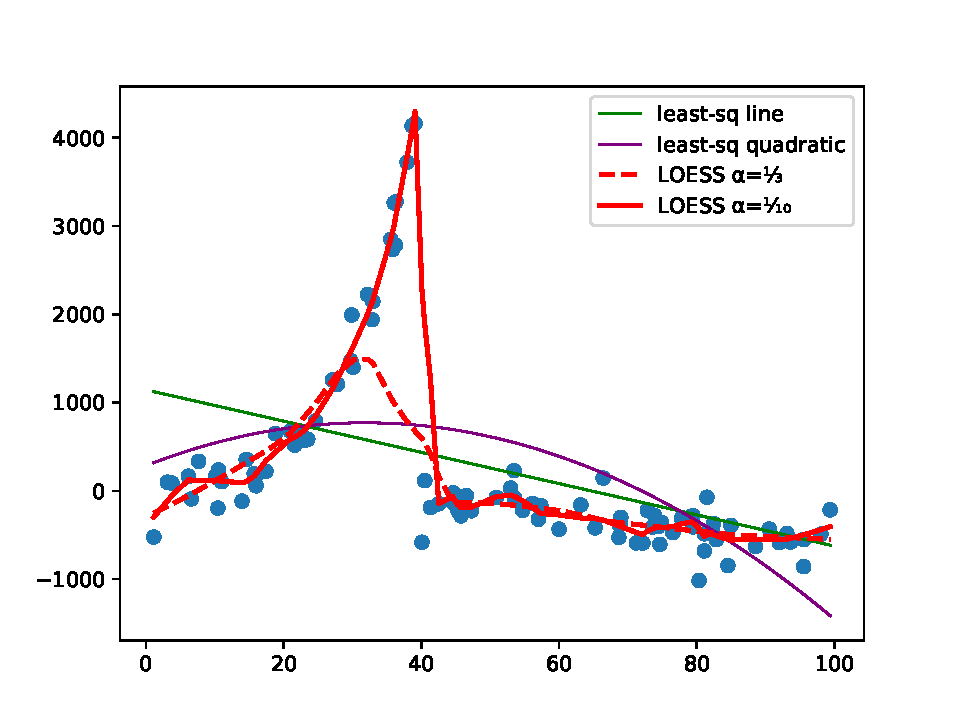
\includegraphics[width=.95\textwidth,
  alt={Scatter plot of about 100 blue points that hover near 0 for x below 20, rise sharply to a spike of about 4000 just before x = 40, then drop back to around -300 and drift slightly downward to x = 100. The green line and purple quadratic miss the spike entirely; the dashed red LOESS with alpha one third rises only to about 1500; the solid red LOESS with alpha one tenth follows the spike almost exactly.}]{lowess_better.pdf}
\caption{A decidedly non-linear data set, for which LOWESS (and particularly
LOWESS with a low $\alpha$) does quite well.}
\label{fig:lowessBetter}
\end{figure}

\medskip
In general, LOWESS is a better \textit{exploratory} technique than best-fit
parametric curves are. This is true for a couple of reasons:

\begin{compactitem}
\itemsep.5em
\item When exploring a data set, you're looking for patterns that stick out,
and you want to let the data speak for itself. You're not coming to the data
with a pre-established model choice and wanting to fit it. LOWESS lets you be
model-agnostic and yet see the forest instead of just trees.

\item LOWESS (and non-parametric methods in general) are ``robust,'' meaning
they aren't as adversely affected by outliers. Consider fitting a least-squares
line to a set of data, and then introducing a couple of outliers near one of
the far ends. This is going to force your global-error-minimizing best-fit line
to swing radically away from the bulk of the data (which it may describe fairly
adequately) in order to try and reach those outliers. Clearly this isn't a good
fit for the data! LOWESS, however, will only ``reach'' for those outliers in
the $x$ range when it gets near those outliers.

% TODO: add plot to demonstrate the above paragraph.

\end{compactitem}

\vspace{.1in}

By the way, although we fit a \textit{linear} function to each local point, we
could fit a quadratic, cubic, or anything else. Here's something to think
about: if we replaced the linear ``$mx+b$'' function with just a constant
``$b$'', then LOWESS becomes simply a weighted moving average. Oooo, deep.

\vspace{.1in}

Finally, remember to play with the $\alpha$ parameter just as you played with
the kernel width and bin size in other exploratory techniques. Remember:
changing this will give you different views on the data, and different views
are good.